\documentclass[tikz,border=8pt]{standalone}
% Shared TikZ style for synorg platform diagrams. Each diagram \input's this
% inside a standalone document. Palette tracks the Material "teal" site theme so
% figures read as one system in light mode (SVGs are theme-neutral otherwise).
\usetikzlibrary{arrows.meta,positioning,shapes.geometric,fit,backgrounds,calc,decorations.pathreplacing}

\definecolor{synteal}{HTML}{00897B}   % primary
\definecolor{synfill}{HTML}{E0F2F1}   % light fill
\definecolor{synamber}{HTML}{B26A00}  % warning / lend
\definecolor{synred}{HTML}{B00020}    % deny / danger
\definecolor{syngrey}{HTML}{5F6368}   % muted

\tikzset{
  >=Stealth,
  font=\sffamily\small,
  box/.style={draw=synteal,line width=0.6pt,rounded corners=2pt,fill=synfill,
              inner sep=5pt,align=center},
  plane/.style={draw=synteal,line width=0.8pt,rounded corners=3pt,fill=synfill,
                inner sep=8pt,align=center},
  state/.style={draw=synteal,line width=0.7pt,circle,fill=synfill,inner sep=3pt,
                minimum size=11mm,align=center,font=\sffamily\footnotesize},
  decision/.style={draw=synteal,line width=0.7pt,diamond,aspect=2,fill=synfill,
                   inner sep=1pt,align=center,font=\sffamily\footnotesize},
  deny/.style={draw=synred,fill=synred!8,text=synred},
  warn/.style={draw=synamber,fill=synamber!10},
  flow/.style={->,line width=0.6pt,draw=syngrey},
  flowlbl/.style={font=\sffamily\footnotesize,text=syngrey,inner sep=2pt},
  note/.style={font=\sffamily\footnotesize\itshape,text=syngrey},
}

\begin{document}
% The R8 region predicate (region-set.md): a candidate region is admitted iff all
% three hold (logical AND). The triple intersection is the eligible set; any one
% circle failing disqualifies the region.
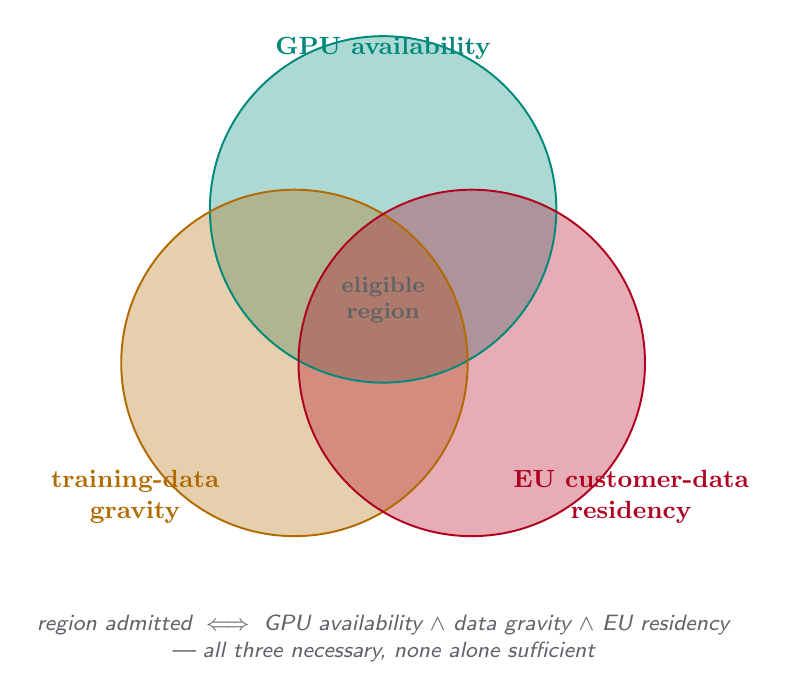
\begin{tikzpicture}
  \coordinate (A) at (90:1.3);   % GPU availability
  \coordinate (B) at (210:1.3);  % training-data gravity
  \coordinate (C) at (330:1.3);  % EU residency

  \begin{scope}[fill opacity=0.32]
    \fill[synteal]  (A) circle(2.2);
    \fill[synamber] (B) circle(2.2);
    \fill[synred]   (C) circle(2.2);
  \end{scope}
  \draw[draw=synteal,line width=0.7pt]  (A) circle(2.2);
  \draw[draw=synamber,line width=0.7pt] (B) circle(2.2);
  \draw[draw=synred,line width=0.7pt]   (C) circle(2.2);

  % set labels, pushed outside their circles
  \node[text=synteal,font=\small\bfseries]  at (0,3.35)   {GPU availability};
  \node[text=synamber,font=\small\bfseries,align=center] at (-3.15,-2.35) {training-data\\gravity};
  \node[text=synred,font=\small\bfseries,align=center]   at (3.15,-2.35)  {EU customer-data\\residency};

  % the admitted set
  \node[align=center,font=\footnotesize\bfseries,text=syngrey] at (0,0.15)
    {eligible\\region};

  \node[note,align=center] at (0,-4.15)
    {region admitted $\iff$ GPU availability $\wedge$ data gravity $\wedge$ EU residency\\
     --- all three necessary, none alone sufficient};
\end{tikzpicture}
\end{document}
